% ==============================================
% ELEMENTOS PÓS-TEXTUAIS
% ==============================================
\postextual
% ||||||||||||||||||||||||||||||||||||||||||||||
% REFERÊNCIAS BIBLIOGRÁFICAS
% ||||||||||||||||||||||||||||||||||||||||||||||
%\bibliography{bibfile2}
% bibliografia john
\bibliography{ref-bibliografica}
% ----------------------------------------------
% Glossário
% ----------------------------------------------
% Consulte o manual da classe abntex2 para orientações sobre o glossário.
%
%\glossary
% ||||||||||||||||||||||||||||||||||||||||||||||
% APÊNDICES
% ||||||||||||||||||||||||||||||||||||||||||||||
% Imprime uma página indicando o início dos apêndices
%\partapendices
% ----------------------------------------------
% Apêndice
% ----------------------------------------------
\begin{apendicesenv}
    \chapter{Avaliação da Aprendizagem}\label{apend-a}
    \begin{enumerate}
    \item O que é a educação financeira?
    
    \item Qual as características de um bom orçamento financeiro?
    
    \item Considerando a Educação Financeira e a Matemática Financeira assinale a alternativa correta:
        \begin{enumerate}
            \item  (   ) A Educação Financeira promove reflexão sobre a vida financeira.
           \item   (   ) A Matemática Financeira trata sobre hábitos financeiros.
            \item  (   ) A Matemática Financeira aborda os tipos de investimentos.
            \item  (   ) A Educação Financeira e a Matemática Financeira são sinônimos.
        \end{enumerate}
    
    \item Selecione a alternativa correta. O orçamento pessoal ou familiar auxilia:
        \begin{enumerate} 
            \item (   ) No controle de receitas e despesas
            \item (   ) Administrar os recursos financeiros de forma consciente
            \item (   ) No controle das dívidas
            \item (   ) Todas as alternativas anteriores
        \end{enumerate}
        
    \item Abaixo há uma lista de itens relacionados às necessidades, desejos e desperdício. Assinale as alternativas referentes somente às necessidades, pode-se escolher mais de uma alternativa.
        \begin{enumerate}
            \item (   ) Sapato de marca - Cirurgia plástica
            \item (   ) Passagem de ônibus - Remédio
            \item (   ) Restaurantes - Viagens - Carro do ano
            \item (   ) Aluguel da casa - Roupas - Lazer
        \end{enumerate}
    
    \item Escolha a alternativa abaixo que representa a ordem das etapas de um Orçamento Financeiro.
        \begin{enumerate}
            \item (   ) Avaliar, Agrupar, Planejar e Registrar
            \item (   ) Registrar, Planejar, Avaliar, Agrupar
            \item (   ) Planejar, Registrar, Agrupar e Avaliar
            \item (   ) Registrar, Agrupar, Planejar e Avaliar
        \end{enumerate}
    
    \newpage    
    \item Qual o tipo de juros é utilizado para rentabilidade dos investimentos?
        \begin{enumerate}
            \item (   ) Juros Simples
            \item (   ) Juros de Mora
            \item (   ) Juros Compostos
            \item (   ) Juros de Capital Próprio
        \end{enumerate}
        
    \item Considerando que a inflação é a variação mensal dos preços, marque a alternativa que representa o índice oficial que o governo brasileiro utiliza para medir a inflação nacional.
        \begin{enumerate}
            \item (   ) CDI
            \item (   ) SELIC
            \item (   ) CDB
            \item (   ) IPCA
        \end{enumerate}
        
    \item Investimento é aplicação do dinheiro poupado para obtenção de juros ou dividendos. Eles possuem três característica Risco, Rentabilidade e Liquidez. Sabendo disso assinale a alternativa que corresponde a definição de Liquidez.
        \begin{enumerate}
            \item (   ) É a probabilidade de ocorrer perdas no investimento
            \item (   ) É a possibilidade do investimento ser transformado em dinheiro
            \item (   ) É a remuneração recebida pelo investimento
        \end{enumerate}
        
    \item Assinale a alternativa cujo investimento não é garantido pelo FGC.
        \begin{enumerate}
            \item (   ) Tesouro Direto
            \item (   ) LCI/LCA
            \item (   ) CDB
            \item (   ) Poupança
        \end{enumerate}
        
    \item Assinale a características de um Investimento em Renda Variável.
        \begin{enumerate}
            \item (   ) Esse tipo de investimento não possui riscos 
            \item (   ) A rentabilidade desse investimento é garantida
            \item (   ) Esse tipo de investimento possui riscos
            \item (   ) É coberto pelo Fundo Garantidor de Crédito
        \end{enumerate}
\end{enumerate}

    
    \chapter{Avaliação do Curso}\label{apend-b}
    \begin{enumerate}
    \item O que te motivou a participar deste curso?
    
    \item Você conhecia os temas abordados nas aulas antes do curso? Se sim, quais temas?
    
    \item Você considera os temas abordados nas aulas importantes para o seu futuro?
    
    \item Os simuladores, jogos (físicos e digitais) e os ambientes virtuais auxiliaram na compreensão dos assuntos abordados durante as aulas? Caso sim de qual forma?
    
    \item Você tem interesse em buscar de novos conhecimentos sobre os temas abordados nas aulas?
    
    \item Você conversou com sua família ou amigos ou parentes sobre o curso? Se sim com quem e quais temas?
    
    \item Quais os temas do curso que mais gostou?
    
    \item O curso está atendendo as suas expectativas.
        \begin{enumerate}
            \item Concordo Totalmente
            \item Concordo Parcialmente
            \item Indiferente
            \item Discordo Parcialmente
            \item Discordo Totalmente
        \end{enumerate}
    
    \item Há alguma sugestão de melhoria, elogio e/ou crítica que gostaria de fazer em relação ao curso?
\end{enumerate}
    
    \chapter{Aplicação do Conhecimento}\label{apend-c}
    Em relação à sua vida financeira atual responda às seguintes perguntas:
\begin{enumerate}
   \item Quais as fontes de dinheiro você utiliza para comprar produtos ou serviços? (Ex: trabalho, estágio, bolsa de estudo, auxílio escolar, mesada, dinheiro dado pelos responsáveis quando necessita, pensão etc).
   
   \item A sua participação no curso de Educação Financeira proporcionou quais mudanças em sua vida e de sua família?
   
   \item De que forma o conhecimento adquirido no curso está auxiliando você e sua família a enfrentar os problemas financeiros causado pela pandemia do COVID-19?
   
   \item Como normalmente você realiza a compra de produtos e serviços?
        \begin{enumerate}
            \item Compro por impulso quando tenho dinheiro para comprar à vista
            \item Compro por impulso e parcelo no cartão de crédito
            \item Planejo, pesquiso e economizo dinheiro antes de comprar à vista
            \item Planejo, pesquiso antes de comprar parcelado no cartão
            \item Outros:
        \end{enumerate}
        
    \item Como você controla suas receitas e gastos mensais?
        \begin{enumerate}
            \item Não anoto nenhum gasto ou receita mensal
            \item Registro todos os gastos e receitas que possuo
            \item Registro apenas gastos e receitas grandes
            \item Outros:
        \end{enumerate}
        
    \item Você separa parte do dinheiro recebido para investir?
        \begin{enumerate}
            \item Sim, antes de gastar
            \item Sim, se sobrar
            \item Não, sempre utilizo todo dinheiro que ganho
            \item Outros:
        \end{enumerate}
    
    \item Normalmente em qual tipo de investimento você aplica o dinheiro poupado? (É possível marcar mais de uma opção).
        \begin{enumerate}
            \item Não poupo dinheiro para aplicar
            \item Caderneta de poupança
            \item Outros investimentos de renda fixa
            \item Investimentos de renda variável
            \item Outros:
        \end{enumerate}
        
    \item Você planeja e economiza parte do dinheiro recebido para sonhos e objetivos futuros?
        \begin{enumerate}
            \item Não, vivo apenas o presente
            \item Não, pois nunca sobra dinheiro
            \item Sim, tenho metas, poupo e aplico dinheiro para objetivos futuros
            \item Outros:
        \end{enumerate}
\end{enumerate}
    
    \chapter{APLICAÇÃO DO CONHECIMENTO - RESPOSTAS}\label{apend-d}
    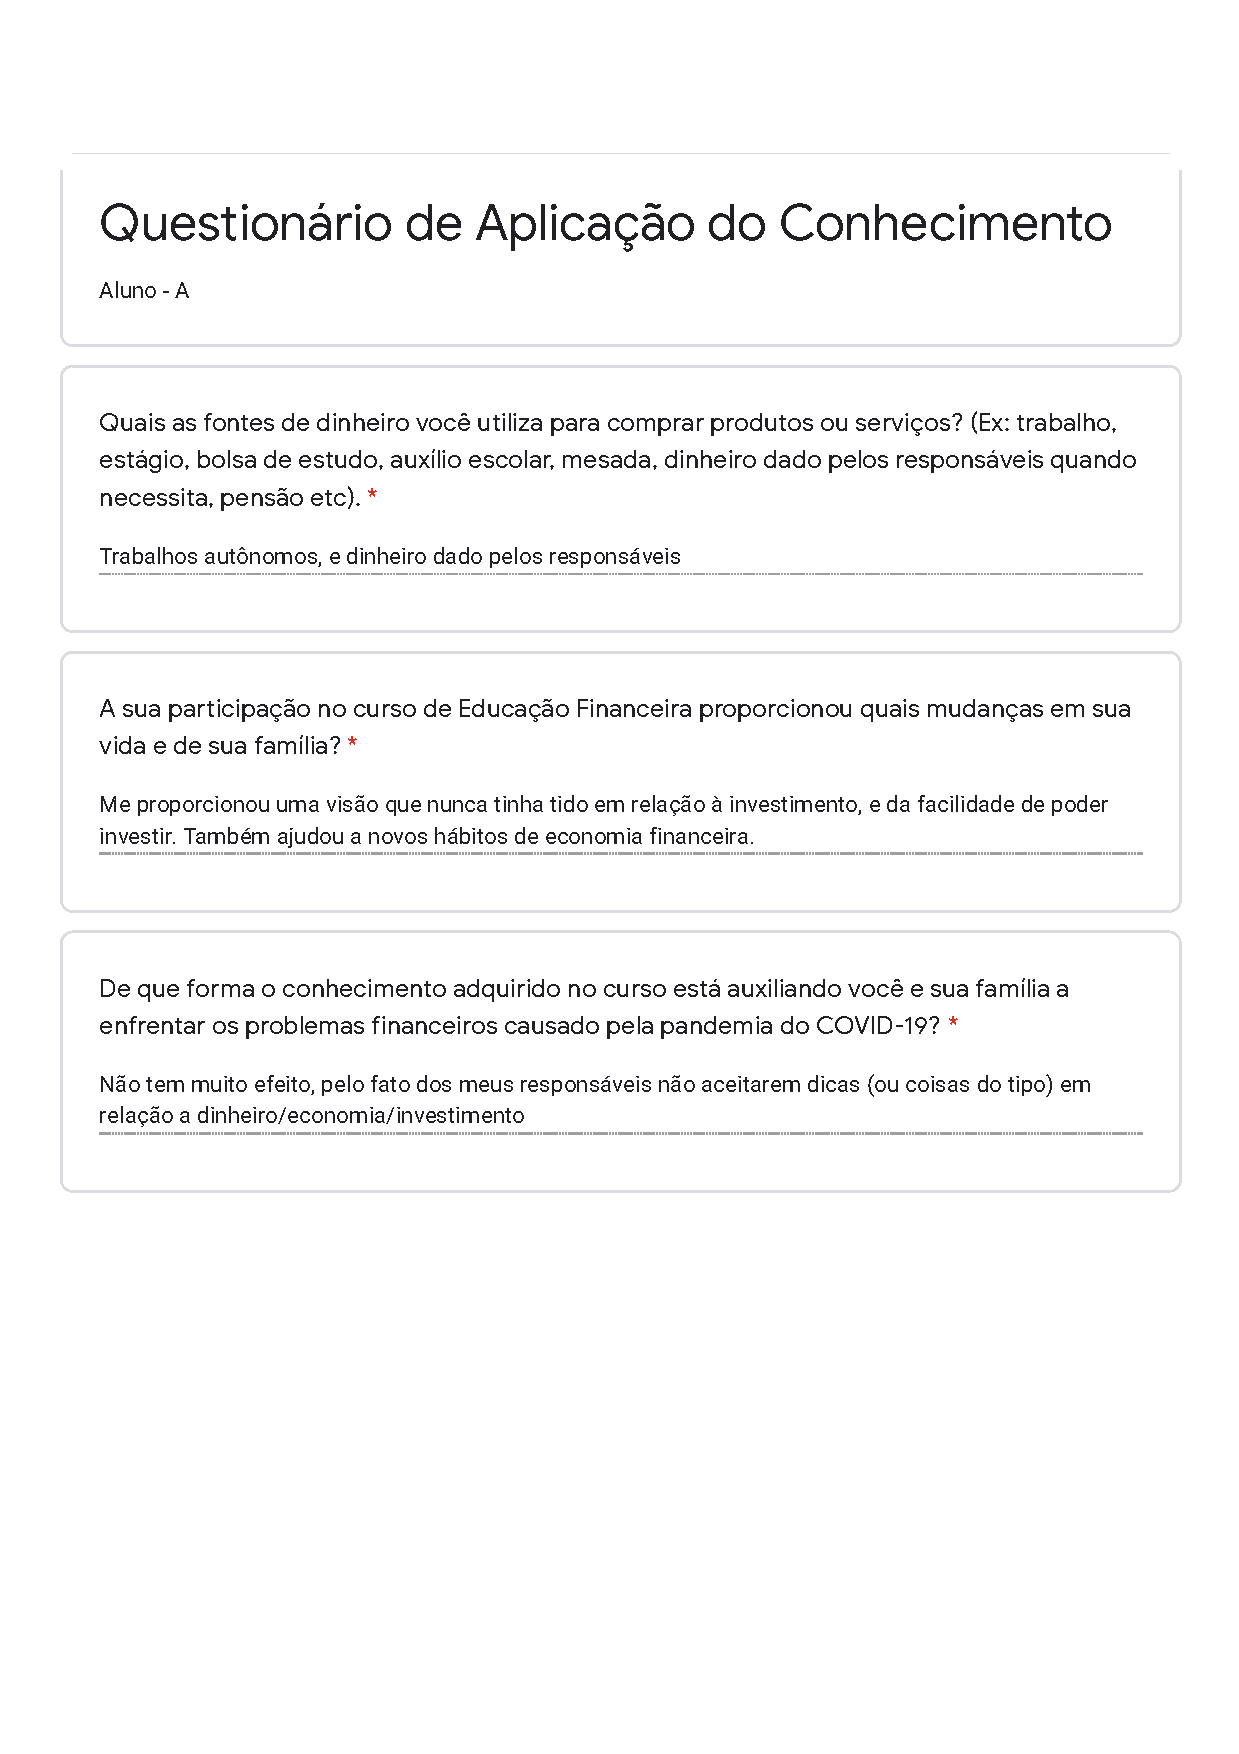
\includepdf[pages=-]{apendices/aplicacao-conhecimento-resposta.pdf}
    
%\includepdf[pages=-]{apendices/apendice.pdf}

\end{apendicesenv}

% ||||||||||||||||||||||||||||||||||||||||||||||
% ANEXOS
% ||||||||||||||||||||||||||||||||||||||||||||||
%\begin{anexosenv}
% Imprime uma página indicando o início dos anexos
%\partanexos
% ----------------------------------------------
% Anexo 1
% ----------------------------------------------
%\chapter{Datasheet}\label{anexo1}
%\includepdf[pages=-]{pdfs/Datasheet.pdf}
% ----------------------------------------------
% Anexo 2
% ----------------------------------------------
%\chapter{Anexo 2}
%\end{anexosenv}
% ==============================================
% INDICE REMISSIVO
% ==============================================
\phantompart
\printindex
% ----------------------------------------------
% ||||||||||||||||||||||||||||||||||||||||||||||
% DOCUMENTO PARA ENTREGA VERSÃO FINAL
%||||||||||||||||||||||||||||||||||||||||||||||
\begin{comment}

\clearpage\thispagestyle{empty}\addtocounter{page}{-1}
\section*{ENTREGA DA VERSÃO FINAL DE DISSERTAÇÃO}

\vspace*{2cm}
Eu, \textsc{\imprimirorientador}, autorizo o aluno(a) \textsc{\imprimirautor} a entregar a versão final da dissertação de mestrado, à secretaria do MPIE, que foi por mim analisada e está de acordo com os apontamentos feitos pelos membros da banca de apresentação do referido aluno.

\vspace*{1cm}
\begin{center}   
   \assinatura{{\imprimirorientador} \\ Orientador}
\end{center}

\vspace*{1cm}
\begin{flushright}
	\imprimirlocal, 11 de Julho de \imprimirdata.
\end{flushright}
\clearpage
\end{comment}
